%------------------------------------------------------------------------------
% $Id: easychair.tex,v 1.23 2008/06/22 17:55:18 mokhov Exp $
%

% Select appropriate paper format in your document class as
% instructed by your conference organizers.
%
% The available formats are 'letterpaper' and 'a4paper' with
% the former being the default if omitted as in the example
% below.
%
\documentclass{easychair}
%\documentclass[a4paper]{easychair}

% In order to save space or manage large tables or figures in a
% landcape-like text, you can use the rotating and pdflscape
% packages. Uncomment the desired from the below.
%
% \usepackage{rotating}
% \usepackage{pdflscape}
%
\usepackage{import}
\usepackage{epstopdf}
\usepackage{bsymb}
\usepackage{alltt}
\usepackage{amsmath}
\usepackage{amssymb}
\usepackage{multicol}
% If you plan on including some algorithm specification, we recommend
% the below package. Read more details on the custom options of the
% package documentation.
%
% \usepackage{algorithm2e}

% Some of our commands for this guide.
%
\newcommand{\easychair}{\sf{easychair}}
\newcommand{\miktex}{MiK{\TeX}}
\newcommand{\texniccenter}{{\TeX}nicCenter}
\newcommand{\makefile}{\texttt{Makefile}}


\makeatletter
\newenvironment{tablehere}
  {\def\@captype{table}}
  {}

\newenvironment{figurehere}
  {\def\@captype{figure}}
  {}
\makeatother


%% Document
%%
\begin{document}

%% Front Matter
%%
% Regular title as in the article class.
%
\title{From Event-B Models to Code}

% \titlerunning{} has to be set to either the main title or its shorter
% version for the running heads. Use {\sf} for highliting your system
% name, application, or a tool.
%
\titlerunning{Event-B Code Generation}

% For only the editors. Authors, please keep this commented out
%\volumeinfo
%	{} % editors
%	{}                         % number of editors
%	{}    % event
%	{}                         % volume
%	{}                         % issue
%	{}                         % starting page number

% Authors are joined by \and and their affiliations are on the
% subsequent lines separated by \\ just like the article class
% allows.
%

\author{Andrew Edmunds\\
School of Electronics and Computer Science,\\
University of Southampton, UK\\
\url{ae2@ecs.soton.ac.uk}\\
\and
Michael Butler\\
School of Electronics and Computer Science,\\
University of Southampton, UK\\
\url{mjb@ecs.soton.ac.uk}\\
}

% \authorrunning{} has to be set for the shorter version of the authors' names;
% otherwise a warning will be rendered in the running heads.
%

\authorrunning{Edmunds and Butler.}

\maketitle

%------------------------------------------------------------------------------
% Abstract
%
\begin{abstract}
Event-B is a formal approach to modelling systems, based on set theory, predicate logic and arithmetic. To make developments tractable, various techniques are used, including refinement, and decomposition. This article describes an extension to the Event-B approach, which we call Tasking Event-B, that facilitates automatic generation of source code from annotated Event-B models. We believe that automatic code generation makes a useful contribution to the Rodin tool-set; by contributing a link in a coherent tool-chain. To validate the approach we have undertaken case studies and taken part in an industrial collaboration. We present a number of case-studies to illustrate our work, in this article.
\end{abstract}

\section{Introduction}
Event-B~\cite{ABR10} is one of a number of formal methods that may be used to model systems where a high degree of reliability is required. Event-B was inspired by its predecessor, \emph{Classical-B}~\cite{TheBBook}. It is a modelling language, used with a supporting tool platform, Rodin~\cite{abrial10rodin}; so named from the project in which it was developed~\cite{RodinTool}.  

In this section we introduce Event-B to the reader, and compare Event-B with some other formal approaches. We discuss automatic code generation from formal models, and potential target programming languages.

In Sect.~\ref{} we...
In Sect.~\ref{} we...

\subsection{Event-B}
The formal methods related to the work presented here can be categorized as state-based formal methods. Alternative, but not unrelated, approaches are categorized as process-based methods. Classical-B~\cite{TheBBook,CNP,CNPInterface,B4Free} and its successor, Event-B are said to be state-based, since they focus on modelling the changes of state, not the behaviour of processes. In Classical-B, state updates are modelled by guarded operations, where the operation is an analogue of a procedure call in a programming language. In Event-B, state updates are modelled by guarded events, providing a more abstract view of the way a system evolves. Event-B can be used to model systems at an abstract level; and by adding more detail (using a technique called refinement) it can model the software aspects of systems too. Both methods are set theoretic modelling approaches that incorporate a notion of proof to show that important system properties are maintained. The former is primarily an approach to software systems development, the latter more widely applicable to system-modelling. In an effort to make modelling and proof easier, Event-B was developed to overcome some of the difficulties encountered when using in Classical-B. The main differences between Classical and Event-B are highlighted in~\cite{Hallerstede07}, and inspiration was also drawn from action systems~\cite{Back1990133}.

It is fair to say that Event-B is not just a formal modelling language; the name is used to describe both a notation, and a methodology. In addition to this a mature tool-platform called \emph{Rodin}, named after its development programme, complements the methodology. The main modelling components of Event-B are contexts and machines. Contexts are used to model static features using sets, constants, and axioms. Machines are used to model variable state using \emph{variables}. A third, more recent addition, is the Theory component; where a developer can augment the bundled mathematical language, and rule-base, with new (inference and re-write) rules, data types, and operators. During the modelling process, changes to the components result in automatic generation of proof obligations, which must be discharged in order to show that the development is consistent. The proof obligations generated in classical-B are often complex, the Event-B approach results in simpler proof obligations as described in~\cite{Hallerstede07}, since Event-B consists of a simplified action syntax, giving rise to simpler proof obligations. A further simplification was made by adopting an event-based approach, where each atomic event has a predicate guard and an action consisting only of assignment statements. Events correspond to operations in the B-method; operation specification was more expressive, and included constructs for specifying operation preconditions (as part of its Design by Contract approach), operation calls, return parameters, and more complex structures for branching and looping. These constructs are not features of Event-B. Due to these simplifications (and more efficient proof tools) a large number of the proof obligations may be discharged automatically, by the automatic provers. Where un-discharged proof obligations remain, the user has, at their disposal, an interactive prover. Various techniques can be applied, to discharge the proof obligations, such as adding hypotheses; or making use of the hyperlink-driven user interface, for rule and tactic application. 

As we mentioned earlier in the section, Event-B makes use of a technique called refinement, where a machine can be refined by another. During this process new variables, events and invariant properties can be added; or existing events can be modified, but in a restricted manner. Machine refinement is transitive and leads to a hierarchical structure. Refinements are related to their more abstract counterparts in such a way that, a valid refinement always satisfies the specifications higher in the refinement hierarchy. In this way, important system properties can be specified at a high level of abstraction, and maintained down through the refinement chain. The Event-B tools are responsible for generating the proof obligations relating to refinement; these must be discharged in a similar way to those generated for proof of machine consistency. In some cases we may model entities in an abstraction that are defined in the event parameters; and in the refinement these entities may be introduced to the model as machine variables. To assist with the proof effort, we can link the parameters of the abstract event with their concrete counterpart using a $WITNESS$, this construct is a predicate describing the relationship between the event parameter of the abstraction and a corresponding variable in the refinement. It is often necessary to specify a linking invariant, to describe the relationship between the variables of the abstract and refinement machines. Inspection of the proof obligations can assist in this task since some of the un-discharged proof obligations provide information about this link. Another feature of Event-B is the ability to  refine one atomic event with a number of events, thus breaking the atomicity, as described in~\cite{Butler08}. Eventually, at the end of a refinement chain the models are detailed enough to accurately describe an implementation. But Event-B is a modelling language, and there is a disjunction between the description of the system in Event-B, and commonly used programming languages, such as Java, C and Ada. Addressing the semantic gap between Event-B and programming constructs is the subject of this article, which we will introduce fully, later in the article.

In terms of the recommended methodology, Event-B development begins with the abstraction, and modelling, of the observable events occurring in a system. Event-B (corresponding to its name) takes an event-based view of a system. The event-based approach uses guarded events to describe the observable events. An event is said to be enabled when the guard is true, and the state updates, described in the event actions, can take place; otherwise it is disabled, and none of its updates can occur.  An example of an Event-B machine can be seen in Fig.~\ref{fig:controllerSpec2}. It shows an abstract model of a pump controller, used in one of the case studies. We will use this model to describe some features of Event-B. But first we introduce the case study, which models a discrete \emph{pumpController}. The model describes a system where the controller receives a value of the fluid level, and a boolean value representing a user-request to turn the pump. Based on the inputs to the controller, a command to turn the pump on may be issued, or a warning is issued if a minimum level \emph{MIN} has been reached.    
%
%
%
\begin{figure}
\centering
\begin{minipage}{0.95\textwidth}
\textcolor{blue}{MACHINE} m1 \textcolor{blue}{REFINES} m0 \textcolor{blue}{SEES} ctx \\
\textcolor{blue}{VARIABLES} \text{m\_level, c\_level, e\_level, m\_pumpOnReq, c\_pumpOnReq, e\_pumpOnReq,} \hspace*{0.2cm} m\_pumpOnCmd, c\_pumpOnCmd, e\_pumpOnCmd, m\_warn, c\_warn, e\_warn,\\
\hspace*{0.2cm} c\_level\_internal, c\_pumpOnReq\_internal\\
\textcolor{blue}{INVARIANTS}\\
\hspace*{0.2cm}(c\_level\_internal $\leq$ MIN $\land$  c\_pumpOnReq\_internal = TRUE $\limp$  c\_warn = TRUE)\\
\hspace*{0.2cm} $\land$ (c\_level\_internal $>$  MIN $\land$  c\_pumpOnReq\_internal = TRUE\\
\hspace*{0.5cm} $\limp$  c\_pumpOnCmd = TRUE)\\
\hspace*{0.2cm} $\land$ (c\_level\_internal $\in  \intg$)\\
\hspace*{0.2cm} $\land$ (c\_pumpOnReq\_internal $\in$  BOOL) \ldots\\
\textcolor{blue}{EVENTS}\\
\textcolor{blue}{INITIALISATION} c\_level :=  100 $\pprod$ m\_level := 80 $\pprod$ c\_pumpOnReq :=  FALSE $\pprod$ \ldots\\
\textcolor{blue}{EVENT} fmiSetBoolean\_c \textcolor{blue}{REFINES} fmiSetBoolean\_c\\
\hspace*{0.2cm}\textcolor{blue}{ANY} p\\
\hspace*{0.2cm}\textcolor{blue}{WHERE} p = c\_compound $\land$ p $\in$ BOOL  \\
\hspace*{0.2cm}\textcolor{blue}{THEN} m\_pumpOnCmd :=  p\\
\hspace*{0.2cm}\textcolor{blue}{END}\\
\ldots
\end{minipage}
\caption{An Event-B  Pump Controller Model}
\label{fig:controllerSpec2}
\end{figure}
%
%
%
 In Fig.~\ref{fig:controllerSpec2}, we see that machine \emph{M1} refines another machine, \emph{M0}. It also has a \emph{SEES} clause, to make the contents of a context visible. The context may contain sets, constants, axioms and theorems. There are variables representing the internal state of the controller, and invariants providing type information for variables. Invariants are also used to describe the safety properties of the system. This describes a required safety property, that if the level is at or below \emph{MIN}, and a user's pump-on request is detected, then a warning will be issued. Also, if the level is OK and a pump-on is requested, then the state \emph{pumpOnCmd = TRUE} is  set.  Following the \emph{INVARIANTS} clause are the model's \emph{Events}. The \emph{Initialisation} event is special event, since it has no guards. The initialisation event of a machine must occur before any other event in the machine is enabled. The event in the figure has a parameter \emph{p}, in the \emph{ANY} clause. Parameters can be used to represent information flow, in and out of events, or they can represent a \emph{local} variable within the scope of the event. The event guard is defined in the \emph{WHERE} clause, in the example, where \emph{p} is typed as a Boolean. The guard relates the parameter to a machine variable \emph{c\_pumpOnCmd}, in the predicate $ p = c\_compound$. The event action appears in the \emph{THEN} clause, where the parameter is assigned to the variable \emph{m\_pumpOnCmd}, in the expression $m\_pumpOnCmd := p$.

---




-----
-----

%
%
%
One important aspect of the Event-B approach is that $any$ enabled event may occur, but only one of the enabled events may occur at any one moment. When modelling certain aspects of a system we may wish to impose an ordering of events. However, there is no sequence operator provided in the Event-B approach. It is therefore necessary to make appropriate use of guards and and state variables to model this aspect of a system. For example if we wish to impose an ordering on two events \emph{evt1} and \emph{evt2} so that $evt1$ occurs before $evt2$ we can use the following approach. Introduce an enumerated set $Grds = \{one,~ two,~ stop\}$ and a variable $step~\in~Grds$. Initially $step~\bcmeq~one$; and we make use of $step$ in the event guards as follows,
\begin{equation}
\begin{split}
&evt1 = \textbf{WHEN}~ step = one~ \textbf{THEN}~\ldots\pprod step \bcmeq two~ \textbf{END}\\
&evt2 = \textbf{WHEN}~ step = two~ \textbf{THEN}~\ldots\pprod step \bcmeq stop~ \textbf{END}\\
\end{split}
\notag
\end{equation}
This ensures that initially $evt1$ is enabled and $evt2$ is disabled since $step = one$; only after $evt1$ has updated the $step$ variable  to $two$ is $evt2$ enabled. At this time $evt1$ is no longer enabled since its guard is now false. Finally no events are enabled since $step = stop$ and all guards are false.


\subsection{Related Approaches}



-- VDM


-- Z
\subsection{Code Generation Rationale}


\subsection{Targets for Code Generation}

- Ada

- Java

- FMI-C


\section{More about Event-B}

\subsection{Decomposition and Composition}

Decomposition and composition are two related approaches, that we use to partition a system, to allow us to work on smaller, manageable sub-models. Figure~\ref{fig:decomp2} illustrates the shared-event decomposition approach~\cite{decomp2010c} which we make use of in our code generation approach. An alternative shared-variable approach is described in~\cite{AbrialH07}. In the shared-event decomposition approach the system is partitioned so that each variable is allocated to a single machine. In the figure, the variables of machine $m$ are partitioned into the sets $v1$ and $v2$ and decomposed into $m_a$ and $m_b$ respectively. The events ....
 %
\begin{figure}
\centering
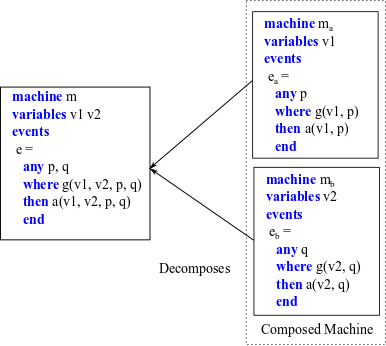
\includegraphics[width=0.5\textwidth]{graphics/Decomp2.png}
\caption{Decomposition}
\label{fig:decomp2}
\end{figure}





\subsection{Theories}

\subsection{ProB}


\section{Tasking Event-B}\label{TEB}
In this section we begin our discussion about Tasking Event-B. We begin by describing the Event-B semantics of the notation. An Event-B model is an abstraction of a system, the evolution of the state is described using events. The guard of an event describes the conditions which must hold prior to an event being enabled. The actions describe the values of the state variables after the event has occurred. Proof obligations are generated, to ensure that the actions update the state with values that satisfy invariant. As a result, a system that is consistent, can be described using events that do not impose an ordering. Since, in Event-B, any enabled event can occur. Now, as we approach the implementation-level specification, we will consider how the behaviour of a task-like implementation construct can be modelled in Event-B, and we will introduce a notation for the purpose of ordering of events. In the following discussion, we distinguish between the behaviour of a task, such as it's life-cycle (which is not modelled formally) and the updates to state (which are modelled formally). In our approach we intend that the implementation-level development be a refinement of the abstract development. We will therefore introduce notations that assist with the formal and non-formal aspects of the specification. The non-formal aspects of the notation are required in the case that we want to generate code for periodic tasks, for instance. 

\subsection{Flow Control for Events}
To enable us to impose sequential order on events we introduce two notions. The first is the \emph{task body}. The task body is an extension to the standard Event-B constructs of variables, events and so on. The task body is a place to specify implementation-level detail using an event ordering notation. The second notion is that of a sequential operator; this is one one the operators that can be used in the task body.

In a model with two events \emph{evt1} and \emph{evt2}, if we wish to order them sequentially, we can write \emph{evt1;evt2} where we use the semi-colon as the sequence operator. To impose an ordering we introduce a Boolean flow control variable for each event. When set to TRUE the event of that name can occur. We see this is Fig.~\ref{fig:seq}. 
%
\begin{figure}
\centering
\begin{minipage}{0.7\textwidth}
Variables evt1, evt2\\
Invariant evt1 $\in \Bool \land$ evt2 $\in \Bool$  \\
Initialisation = evt1 $\bcmeq$ TRUE $\pprod$ evt2 $\bcmeq$ FALSE\\
evt1 = \textbf{WHEN}~ evt1 = TRUE~ \textbf{THEN}~$A_1~ \pprod$ evt1 = FALSE $\\
\hspace*{1.0cm} \pprod$ evt2 = TRUE \textbf{END}\\
evt2 = \textbf{WHEN}~ evt2 = TRUE~ \textbf{THEN}~$A_2~ \pprod$ evt2 = FALSE  \textbf{END}\\
\end{minipage}
\caption{Sequence}
\label{fig:seq}
\end{figure}
Initially $evt1$ is enabled and $evt2$ is disabled, since $evt1 = TRUE$ and $evt2 = FALSE$. The update action $A_1$ occurs, with the control variable updates setting \emph{evt1} to $FALSE$ and $evt2$ to $TRUE$. Therefore the next step is for the event $evt2$ to be enabled, and so on.

T(e_1 ; e_2) =
T(e_1, e_2);T(e_2, _)

e_1 = g_1 \rightarrow a_1



For branching


To the CLM:
In many programming languages we see the semi-colon `;' used as a delimiter, to terminate a program statement. A sequence of program statements is constructed by appending semi-colon delimited statements. In formal languages we often use the semi-colon as an operator. When thinking about a sequence of events we need to consider the relationship between our notion of sequence, and the delimiter used in these languages. An event is an atomic update; so, in a multi-tasking environment, it should be implemented with the necessary protection mechanisms. The CLM isolates us from this.   



\subsection{Theories for TEB}

\subsection{State-machines}

\section{Tooling}

\subsection{The Rodin Platform and Eclipse}

\subsection{IL1/CLM}

\subsection{Templates}

\subsection{Interfaces}

\section{Conclusions}
\subsection{Discussion}

\subsection{Related Work}
As we mentioned in the introduction, the main driver for this work has been to derive the greatest benefit from the formal modelling approach, by making use of the formal modelling artefacts to generate implementations. There are many formal notations and many have support for automatic code-generation.

The Classical-B~\cite{TheBBook} approach made use of an implementation-level notation called \emph{B0}, described in~\cite{B0RefMan}. B0 is similar to a programming language, and consists only of concrete programming constructs. These constructs map to programming constructs in a number of programming languages. \emph{B0} forms part of the Classical-B refinement chain, so the implementation-level specification refines the abstract development. Translators are available targeting programming languages such as C~\cite{KernighanR88}, and $High~ Integrity~ Ada$ (based on $SPARKAda$~\cite{SPARKAda}). 

The \emph{Z-notation} is a state-based specification notation (actually a distant ancestor of Event-B).  

The VDM-SL is a state-based formal specification language, related to $Z$, and has tool support for automatic code generation. 

VDM++ is an object-oriented extension to Models can be described textually; or using a graphical interface using UML diagrams, in much the same way as UML-B does for B and Event-B. VDM++ can be used with the VDM++ Toolbox to generate C++ and Java code. VDM++ can be used to model and implement developments with concurrently executing processes, using threads.

\emph{Object-Z}~\cite{GSmith2000} is an object-oriented approach to development using $Z$. A route to implementation is described using a translation to \emph{PerfectDeveloper}~\cite{PD} in~\cite{Stevens06}. \emph{PerfectDeveloper}'s approach is to use verified-Design By Contract, where verification conditions are generated from a specification using constructs such as pre and postconditions, class and loop invariants, and assertions. The verification conditions must be shown to hold in order to show the specified contracts are satisfied by the implementation. They are generated for each method entry to show that the precondition holds, for each method exit to show that the postcondition holds, and wherever an assertion appears. \emph{PerfectDeveloper} provides automatic, and semi-automatic, translations to Java and C++ but appears not to support concurrent processing.

There are some combined formal approach where code-generation has been investigated. CSP~\cite{HO85CSP,Roscoe1997} is a process algebraic approach to system specification in which the ordering of events occurring in a system play a major role. CSP specifications have been translated into Java code using JCSP~\cite{JCSPNet,JCSPMulti}. A hybrid CSP and Classical-B approach~\cite{SchneiderT02,SchneiderT05} combines the benefits of modelling, using both process-based and state-based techniques.  In this approach, called $CSP\pprod B$, specifications are used to constrain the order that the state-changing operations may occur; and to specify points at which the processes may interleave. The B operations synchronize with CSP events with the same name, and provide an ordering of the occurrence of B operations. ProB~\cite{LeuschelB08} is an animator and model checker for Classical-B and Event-B, and can be used with the $CSP\pprod B$ combination. It is used in the JCSProB~\cite{YangPop2007} approach, which combines CSP and Classical-B, and has a code generator inspired by JCSP. Another combined approach, amenable to model-checking, is \emph{Circus}~\cite{WoodcockC01}, which is combination of CSP and \emph{Z-notation}~\cite{Spivey89}. CSP is used to order the $Z$ operations. It can be translated to Java as described in~\cite{FreitasC06} and makes use of the JCSP library.



%------------------------------------------------------------------------------
% Refs:
%
\label{sect:bib}
\bibliographystyle{plain}
%\bibliographystyle{alpha}
%\bibliographystyle{unsrt}
%\bibliographystyle{abbrv}
\bibliography{MyBibTex}

\end{document}

% EOF
